% prelude latex <<<
\tracingmacros=0
\documentclass{llncs}
% packages <<<
\usepackage[english]{babel}
\usepackage{amsmath}
\usepackage{amssymb}
\usepackage{booktabs}
\usepackage{graphicx}  % TODO: paint everything in tikz and remove this
\usepackage{listings}
\usepackage{mathrsfs}
\usepackage{microtype} % keep even if it seems not to do anything!
\usepackage{tikz}
\usepackage{xcolor}
\usepackage{xspace}
\usepackage[colorlinks]{hyperref}  % solves pdfTeX warning (ext4)?
\usepgflibrary{arrows}
% >>>
% meta <<<
\title{FreeBoogie}
\subtitle{201105}
\author{Radu Grigore\inst{1} and Joseph Roland Kiniry\inst{2}}
\institute{Queen Mary, University of London
\and IT University of Copenhagen}
% >>>
% PDF settings <<<
\definecolor{darkblue}{rgb}{0,0,0.4}
\definecolor{verylightgray}{rgb}{0.9,0.9,0.9}
% comment the next line for printing
\hypersetup{colorlinks,linkcolor=darkblue,citecolor=darkblue,urlcolor=darkblue}
\hypersetup{
  pdfauthor={Radu Grigore and Joseph Kiniry},
  pdftitle={FreeBoogie}}
% >>>
% tikz helpers <<<

% global styles
\tikzstyle{arr}=[->,>=stealth']
\tikzstyle{predcirc}=[
  circle,
  very thick,
  fill=green!10,
  draw=green,
  minimum size=14pt,
  inner sep=0pt]
\tikzstyle{predrect}=[predcirc,rectangle,inner sep=2pt]

% These macros and styles are used for drawing flowgraphs
\newcommand\fgnodeR{2pt}  % the default radius of a flowgraph node
\tikzstyle{fgdraw}=[
  minimum size=2*\fgnodeR,inner sep=0pt,outer sep=1pt,
  draw,thick]
\tikzstyle{fgfill}=[fill=black]
\ifx\fgnode\undefined\else\errmessage{\string\fgnode already defined!}\fi
\def\fgnode#1#2(#3) at (#4){% uses \def because of the special syntax
    \begin{scope}[shift={(#4)},shift only]
      \clip (-\fgnodeR,-#1*\fgnodeR) rectangle (\fgnodeR,#2*\fgnodeR);
      \node[fgdraw,circle,fgfill] {};
    \end{scope}
    \node[fgdraw,circle] (#3) at (#4)}
\newcommand{\oonode}{\fgnode00} % the normal non-reading non-writing node
\newcommand{\ronode}{\fgnode01} % for read-only nodes
\newcommand{\wonode}{\fgnode10} % for write-only nodes
\newcommand{\rwnode}{\fgnode11} % for read-write nodes
\newcommand{\gnode}{\node[fgdraw,circle,fill=gray]}  % gray nodes (ra)
\newcommand{\cnode}{\node[fgdraw,fgfill,rectangle]} % copy nodes
\newcommand{\enode}{\oonode} % empty node
\newcommand{\fnode}{\rwnode} % filled node
% >>>
% package customization <<<
\lstset{
  basicstyle=\scriptsize,
  identifierstyle=\itshape,
  stringstyle=\footnotesize\ttfamily,
  commentstyle=\textup,
  columns=fullflexible,
  numbers=left,
  numberstyle=\tiny,
  mathescape=true,
  boxpos=t,
}
\lstdefinestyle{boogie}{
  morekeywords={procedure,returns,assume,assert,havoc,goto,return,
    int,bool,type,while,if,true,false,function,bool,returns,axiom,
    forall,var}
}
\lstdefinestyle{jml}{
  language=java,
  morekeywords={requires,ensures,old,invariant,forall,exists,axiom,also,
    result,pure,assert,modifies},
  deletekeywords={label}
}
\lstdefinestyle{smt}{
  morekeywords={ite,true,false,BG_PUSH,IFF,FORALL,EQ,NEQ,NOT,TRUE,FALSE,
    IMPLIES}
}
\newcommand{\lstinlinen}{\lstinline[basicstyle=\normalsize]}
\newcommand{\boogieCode}{\lstinline[style=boogie,basicstyle=\normalsize]}
\newcommand{\jmlCode}{\lstinline[style=jml,basicstyle=\normalsize]}
\newcommand{\smtCode}{\lstinline[style=smt,basicstyle=\normalsize]}
\newcommand{\deflang}[1]{\lstnewenvironment{#1}[1][]{\lstset{style=#1,##1}}{}}
\deflang{jml}
\deflang{boogie}
\deflang{smt}
\abovetopsep=1ex % because tabular appears below captions
% >>>
% new commands <<<
\def\fb#1{{\bf #1}} % for introducing acronyms
\newcommand{\csharp}{C$^\sharp$\xspace}
\newcommand{\escjava}{ESC\slash Java\xspace}
\newcommand{\framac}{\hbox{Frama-C}}
\newcommand{\indentline}[1]{\\\leftline{\indent#1}}
\newcommand{\macro}[1]{\texttt{\char`\\#1}}
\newcommand{\jk}[1]{{\small [\textcolor{red}{jk}: #1]}}
\newcommand{\rg}[1]{{\small [\textcolor{red}{rg}: #1]}}
\newcommand{\shell}[1]{\indentline{\texttt{#1}} }
\newcommand{\specsharp}{Spec$^\sharp$\xspace}

%pairs
\newcommand{\startgrammar}{
  \begingroup
  \def\is{&$\to$&}
  \def\|{$\mid$}
  \def\b##1{\textbf{##1}}
  \def\i##1{\textsl{##1}}
  \def\?{$^?$}
  \def\*{$^\ast$}
  \begin{figure}
  \centering
  \scriptsize
  \begin{tabular}{r@{\;}c@{\;}l}
}
\newcommand{\stopgrammar}[2]{
  \end{tabular}
  \caption{#1}\label{#2}
  \end{figure}
  \endgroup
}

\newcommand{\bc}{\begin{figure}\centering\begin{tabular}{c}} % begin codebox
\newcommand{\ec}[2]{\end{tabular}\caption{#1}\label{#2}\end{figure}} % end codebox

% >>>
% TeX settings <<<
\overfullrule=5pt
\showboxdepth=10
\showboxbreadth=100
% >>>
% >>>
% boogie and lncs instructions <<<
% - 12 pages, lncs format
% >>>
\begin{document}
\maketitle
% abstract <<<
\begin{abstract}
We describe the current design of FreeBoogie, a static verifier for Boogie
programs.
\end{abstract}
% >>>
\section{Introduction} % <<<

``Why another static verifier for Boogie? Is there something so wrong with
the one from Microsoft Research that it cannot be fixed?'' We expect that
many readers have these thoughts at this point, so we answer.  FreeBoogie
exists because we wanted to change the Boogie language back in 2007 and
Microsoft's verifier was closed source at the time. We keep FreeBoogie
alive for three main reasons. First, we like the Boogie language and
history shows that languages have higher chances to survive if they have
multiple implementations. Second, the FreeBoogie project has distinct
priorities, namely simplicity of its code and good documentation. Third,
FreeBoogie is easy to compile and use on Linux, because it is written
in~Java.

This paper is written for researchers that want to experiment with the
Boogie language. For example, one might be interested in verifying Boogie
programs by symbolic execution rather than verification-condition
generation; another might be interested in adding the heap to Boogie's
semantics rather than keeping it as a global array; yet another might want
to infer procedure specifications for a set of given implementations. These
are all experiments that could be made by modifying FreeBoogie. The main
technical challenge is then to understand FreeBoogie enough to modify it.
Luckily, its code was written so that it is easy to understand. Even
better, this article gives a high-level overview of the design, and points
to the tricky pieces of code, so that you can get up to speed quickly.

% >>>
\section{An Example Run} % <<<
% @review JRK *want*
\bc
\begin{boogie}
type T;
procedure indexOf(x : T, a : [int] T, al : int) returns (i : int) {
  i := 0;
  while (i < al && a[i] != x) { i := i + 1; }
}
\end{boogie}
\ec{A high-level Boogie version of Figure~\ref{lst:first-boogie}}
{lst:boogie-indexof}

The best way to understand how FreeBoogie works is to run
it on a few examples and ask it to dump its data structures
at intermediate stages. Figure~\ref{lst:boogie-indexof}
shows a Boogie program suitable for a first run. Notice
that the language is not restricted to the core defined in
Chapter~\ref{ch:boogie}. To peek at FreeBoogie's internals
use the command \shell{fb --dump-intermediate-stages=log
example.bpl} assuming that you wrote the content of
Figure~\ref{lst:first-boogie} in the file \texttt{example.bpl}
and that FreeBoogie is correctly installed on your system.
This will create a directory \texttt{log}. The output of each
processing phase of FreeBoogie appears in a subdirectory
of~\texttt{log}. The name of the subdirectory is the name of the
phase.

Such transformation phases include desugaring the \textbf{while}
statement, desugaring the \textbf{if} statement, cutting cycles,
eliminating assignments (Chapter~\ref{ch:passive}), computing
the VC (Chapter~\ref{ch:spwp}). Let us look briefly at the state
of FreeBoogie after \textbf{while} and \textbf{if} statements
are desugared. To do so we could look at the pretty-printed
Boogie code but we can also look at the flowgraph that is dumped
by FreeBoogie in the GraphViz~\cite{ellson2001} format. The
flowgraph is rendered in Figure~\ref{fig:first-boogie}. Such
representations of the internal data structures are very helpful
in understanding FreeBoogie and in debugging it.

\begin{figure}
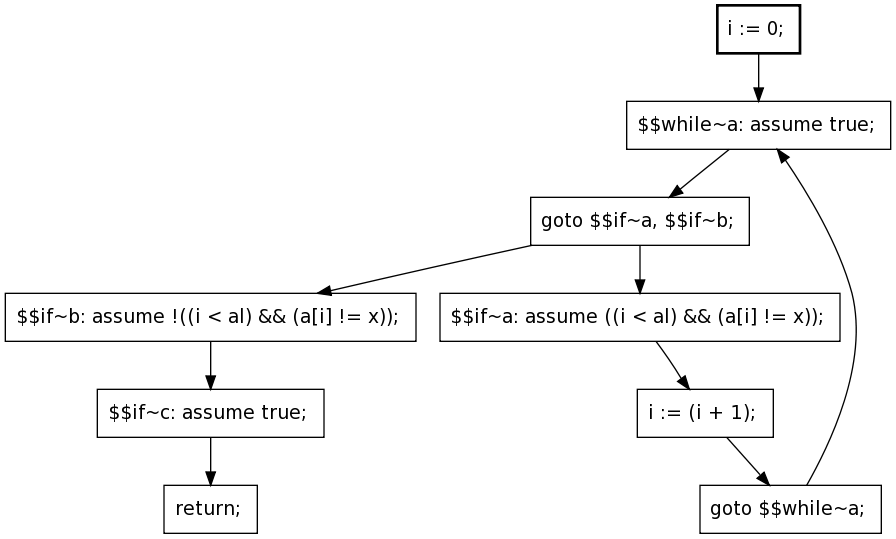
\includegraphics[width=\textwidth]{img/first_boogie.png}
\caption{Flowgraph of a desugared version of Figure~\ref{lst:first-boogie}}
\label{fig:first-boogie}
\end{figure}

The flowgraph is an example of \emph{auxiliary} information that
FreeBoogie computes after each transformation. The other pieces
of auxiliary information are the symbol table and the types. The
\emph{symbol table} is a one-to-many bidirectional map between
identifier definitions and identifier uses. The \emph{types} are
associated with expressions (and subexpressions).

To see the query that is sent to the theorem prover you must
run a different command, this time shown in abbreviated form:
\shell{fb -lf=example.log -ll=info -lc=prover example.bpl} The
log file \texttt{example.log} will contain everything sent to
the prover. The result of the whole run is \shell{OK: indexOf at
example.bpl:2:11} indicating that the program is correct.

% >>>
\section{Pipeline} % <<<
\label{sec:pipeline}
% @review JRK *want*

Figure~\ref{fig:architecture} shows that FreeBoogie has a
pipeline architecture. The \colorbox{green!50!white}{light green}
color stands for the Boogie AST (\fb abstract \fb syntax \fb
tree); the \colorbox{blue!50!black}{\textcolor{white}{dark blue}}
color stands for the SMT AST\null.

\begin{figure} % <<<
  \centering
  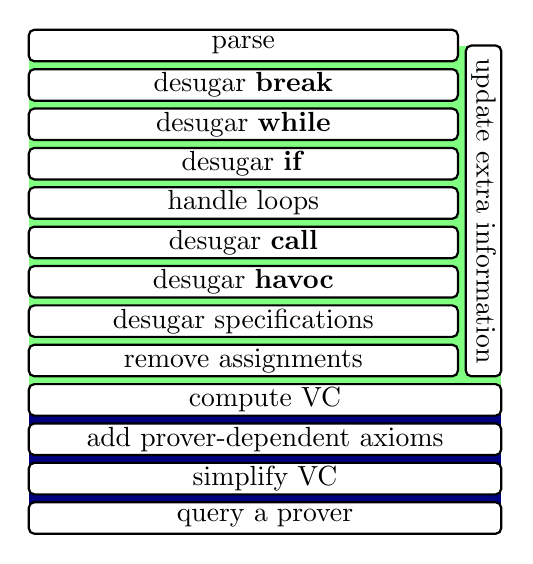
\begin{tikzpicture}[scale=1]
  \tikzstyle phaseS=[thick,rounded corners=2pt,draw=black,fill=white];
  \fill[color=green!50!white] (0,-0.25) rectangle +(6,-4.75);
  \fill[color=blue!50!black] (0,-4.75) rectangle +(6,-1.5);
  \foreach \py/\px/\ptext in {
    0/5.45/parse,
    1/5.45/desugar \textbf{break},
    2/5.45/desugar \textbf{while},
    3/5.45/desugar \textbf{if},
    4/5.45/handle loops,
    5/5.45/desugar \textbf{call},
    6/5.45/desugar \textbf{havoc},
    7/5.45/desugar specifications,
    8/5.45/remove assignments,
    9/6/compute VC,
    10/6/add prover-dependent axioms,
    11/6/simplify VC,
    12/6/query a prover}
  {
    \draw[phaseS]
     [yscale=.5](0,-\py-0.1) rectangle node {\ptext}  +(\px,-.8);
  }
  \draw[phaseS] (5.55,-0.25) rectangle node[rotate=-90] 
    {update extra information} (6,-4.45);

  \end{tikzpicture}
  \caption{FreeBoogie architecture.}
  \label{fig:architecture}
\end{figure} % >>>

Horizontal boxes, except for the first one (parse) and the last
one (query a prover), represent \emph{transformations}. Depending
on the type of input and on the type of output there are three
types of transformations: Boogie to Boogie, Boogie to SMT, and
SMT to SMT\null. For brevity, we say `Boogie transformations'
instead of `Boogie to Boogie transformations', and `SMT
transformations' instead of `SMT to SMT transformations'. All
these transformations are designed not to miss bugs, at the cost
of possible false positives.

\begin{definition}
A Boogie transformation is \emph{sound} when it produces only
incorrect Boogie programs from incorrect Boogie programs. A
Boogie to SMT transformation is \emph{sound} when it produces
only invalid formulas from incorrect Boogie programs. An SMT
transformation is \emph{sound} when it produces only invalid
formulas from invalid formulas.
\label{def:sound-transform}
\end{definition}

\begin{remark}
This definition is in a way formal, but in a way it is not.
It makes use of the concept of `correct Boogie program'
and we only have semantics for \emph{core} Boogie programs
(Chapter~\ref{ch:boogie}). For example, we can say precisely what
it means for the assignment removal transformation to be sound,
because both the input and the output of that transformation are
core Boogie programs; however, we can only informally describe
the preceding transformations as sound.
\end{remark}

The symmetric notion is that of completeness.

\begin{definition}
A Boogie transformation is \emph{complete} when it produces
only correct Boogie programs from correct Boogie programs. A
Boogie to SMT transformation is \emph{complete} when it produces
only valid formulas from correct Boogie programs. An SMT
transformation is \emph{complete} when it produces only valid
formulas from valid formulas.
\label{def:complete-transform}
\end{definition}

All transformations in FreeBoogie are sound; all transformations
in FreeBoogie, except loop handling,
% @review JRK Missing text.

Full Boogie would not be user friendly without high-level
constructs like \textbf{while} statements and \textbf{break}
statements. Many phases in FreeBoogie perform syntactic
desugarings of these constructs. The desugaring is sometimes
local, in the sense that it can be done without keeping track of
an environment, and sometimes it is not. For example, to desugar
the \textbf{break} statement we must keep track of the enclosing
\textbf{while} and \textbf{if} statements; but the desugaring of
a \textbf{havoc} statement does not depend on any surrounding
code.

The most important transformation in FreeBoogie is the
transition from Boogie to SMT\null. The role of preceding Boogie
transformations is to simplify the program to a form on which the
VC is easily computed; the role of subsequent SMT transformations
is to bring the VC to a form that is easily handled by a prover.

The order of Boogie transformations depends on constraints
such as the following. The Boogie to SMT transformation
(`compute VC' in Figure~\ref{fig:architecture}) only handles
the \textbf{assert}, \textbf{assume}, and \textbf{goto}
statements. The Boogie transformation that removes assignments
only handles acyclic flowgraphs. Hence, the flowgraph must
first be transformed into an acyclic one (`handle loops' in
Figure~\ref{fig:architecture}).

The VC uses concepts such as arrays, which may or may not be
known to the prover. In the latter case, axioms that describe
the concept must be added to the VC\null. Finally, the VC is
simplified so that the communication with the prover is
more efficient.

The source code of FreeBoogie, written in Java~6, contains
four packages, which are in one-to-one correspondence with the
following sections.

\begin{itemize}
\item \texttt{freeboogie.ast}: data structures for representing
  Boogie programs and facilities for processing such data structures
\item \texttt{freeboogie.tc}: code that computes auxiliary information
  from a Boogie AST
\item \texttt{freeboogie.vcgen}: the Boogie transformations and
  the Boogie to SMT transformation
\item \texttt{freeboogie.backend}: 
  SMT transformations, 
  data structures for representing SMT, 
  and code for interfacing with the prover
\end{itemize}

% >>>
\section{The Abstract Syntax Tree and its Visitors} % <<<
\label{sec:design.ast}
% @review JRK *want*, but needs a lot of trimming (see below)

The Boogie AST data structures are described using a compact
notation. A subset, corresponding to core Boogie, appears in
Figure~\ref{fig:boogie-absgrm}. AstGen (a helper tool) reads this
description and a code template to produce Java classes. The
approach has advantages and disadvantages. The generated classes
are very similar to each other because they come from the same
template. This means that it is easy to learn their interface.
It also means that it is easier to change all the classes in a
consistent way by changing the template. The compact description
in Figure~\ref{fig:boogie-absgrm} is easier to read than the
corresponding $12$~Java classes. The overall structure of the AST
is easier to grasp. It is also easier to modify, since it takes
far less time to change one or two lines than one or two Java
classes. However, the programmer needs to learn a new language
(the one used in Figure~\ref{fig:boogie-absgrm}) and IDEs are
usually confused by code generators.

\begin{figure}\centering\footnotesize % <<<
\begin{verbatim}
Program = Signature! sig, Body! body;
Signature = String! name, [list] VariableDecl args, [list] VariableDecl results;
Body = [list] VariableDecl vars, Block! block;
VariableDecl = String! name, Type! type;
Block = [list] Statement statements; 
Type = enum(Ptype: BOOL, INT) ptype,
Statement :> AssertAssumeStmt, AssignmentStmt, GotoStmt;
AssertAssumeStmt = enum(StmtType: ASSERT, ASSUME) type, 
  [list] Identifier typeArgs, Expr! expr;
AssignmentStmt = [list] OneAssignment assignments;
GotoStmt = [list] String successors;
Identifier = String! id, 
OneAssignment = Identifier lhs, Expr rhs;
\end{verbatim}
\caption{The abstract grammar of core Boogie}\label{fig:boogie-absgrm}
\end{figure} % >>>

Another consequence of this approach, which might be seen as a
disadvantage, is that there is no way to add specific code to
specific classes: We are forced to implement operations over the
AST using the visitor pattern~\cite{gamma1995}.

\subsection{Visitors} % <<<
\label{sec:visitors}
% @review JRK *not really* (Keep only from *** down, in a tighter revision.)

% @review JRK ***

FreeBoogie uses the traditional visitor pattern and
the root of the visitors' class hierarchy is the class
\jmlCode|Evaluator<R>|. The root of the Boogie AST
class hierarchy is the class \jmlCode|Ast|. A subclass
of \jmlCode|Evaluator<R>| is like a function of type
$\mathit{Ast}\to R$, in the sense that it associates a
value of type~$R$ (possibly \jmlCode|null|) to an AST
node. For example, the type checker is a subclass of
\jmlCode|Evaluator<Type>|. The base class \jmlCode|Evaluator|
declares one \jmlCode|eval($\mathscr{A}$)| method for each AST
class~$\mathscr{A}$. These are the methods called~$m_2$ in the
previous discussion of the general visitor pattern. These methods
are not only declared, but they are also implemented, so that
subclasses explicitly handle only the relevant types of AST
nodes. For all the other AST node types, the default behavior
implemented in \jmlCode|Evaluator| is to recursively evaluate all
children and to cache the results. Because the \jmlCode|eval|
methods of \jmlCode|Evaluator| are so similar, they are generated
from an AstGen template.

An important type of evaluator is a transformer: The class
\jmlCode|Transformer| extends \jmlCode|Evaluator<Ast>|. The
main functionality implemented in \jmlCode|Transformer|, path
copying, is illustrated in Figure~\ref{fig:path-copying}. Empty
nodes (\tikz[baseline=-.5ex] \node[fgdraw,circle] {}; and
\tikz[baseline=-.5ex] \node[fgdraw]{};) represent AST nodes
that exist on the heap before a transformer~$T$ acts; filled
nodes (\tikz[baseline=-.5ex] \node[fgdraw,fgfill,circle]{};
and \tikz[baseline=-.5ex] \node[fgdraw,fgfill]{};) represent
AST nodes created by the transformer~$T$. Because the
transformer~$T$ is interested only in rectangle nodes,
it overrides only the \jmlCode|eval| method that takes
rectangles as parameters. That overriden method is responsible
for creating the filled rectangle (\tikz[baseline=-.5ex]
\node[fgdraw,fgfill]{};). All the other filled nodes
(\tikz[baseline=-.5ex] \node[fgdraw,fgfill,circle]{};) are
created by \textit{Transformer}, and need not be of any concern
to the particular transformer~$T$.

\begin{figure}\centering
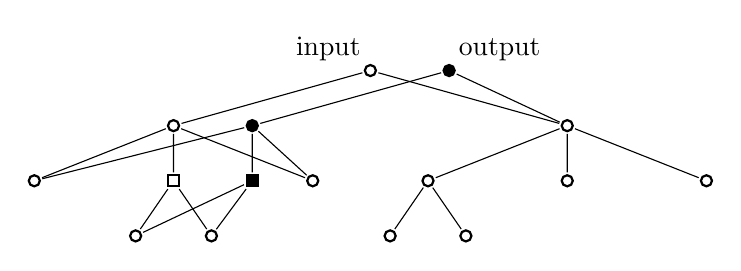
\begin{tikzpicture}
  [level distance=7mm,
  level/.style={sibling distance=5cm/(#1^1.5)}]
\tikzset{tree/.style={fgdraw,circle}}
\node[tree] (A) {}
  child {node[tree] (B) {}
    child {node[tree] (B1) {}}
    child {node[tree,rectangle] (C) {}
      child {node[tree] (C1) {}}
      child {node[tree] (C2) {}}
    }
    child {node[tree] (B3) {}}
  }
  child {node[tree] (A2) {}
    child {node[tree] {}
      child {node[tree] {}}
      child {node[tree] {}}
    }
    child {node[tree] {}}
    child {node[tree] {}}
  };
\path
  (A) +(1cm,0) node[tree,fgfill] (A') {}
  (B) +(1cm,0) node[tree,fgfill] (B') {}
  (C) +(1cm,0) node[tree,fgfill,rectangle] (C') {};
\draw (A') -- (B') -- (C');
\draw (A') -- (A2);
\draw (B') -- (B1); \draw (B') -- (B3);
\draw (C') -- (C1); \draw (C') -- (C2);
\node[above left] at (A) {input};
\node[above right] at (A') {output};
\end{tikzpicture}
\caption{Path copying}\label{fig:path-copying}
\end{figure}

The input and the output of a transformer usually share a large
number of nodes. Since \textit{Evaluator} caches the information
that various evaluators associate with AST nodes, there is no
need to repeat the computation of that auxiliary information for
the shared parts. For example, most of the type information is
already in the cache of the type checker.

Sometimes a transformer wants to `see' AST nodes of type~$A$
even if it computes no value for them. A typical example is
a pretty printer. In such cases a transformer may override
\jmlCode|eval(A)| and return \textbf{null}. A nicer solution is
to override \jmlCode|see(A)|, whose return type is \textbf{void}.
If both \jmlCode|eval(A)| and \jmlCode|see(A)| are overriden,
then the former will be called by the traversal code in
\textit{Transformer}.

% >>>
\subsection{Immutability} % <<<
\label{sec:design.immutability}
% @review JRK *want* (but tighten-up)

In Java programming, it is unusual to constrain data structures
to be immutable. Since the resulting code may look awkward to
many programmers, there better be some good reasons for this
design decision. In fact, awkward code, such as copying all but
one of the fields in a new object instead of doing a simple
assignment, is only one of the apparent problems.

\bc
\begin{jml}
public class Renamer extends Transformer {
  @Override public Identifier eval(Identifier identifier) {
    if (!identifier.id().equals("u")) return identifier;
    else return Identifier.mk("v");
  }
}
\end{jml}
\ec{Changing all occurrences of variable~$v$ into variable~$y$}
{lst:example-transformer}

Immutability implies path copying, which is a
potential performance problem. Consider the task of
changing all occurrences of the variable~$u$ into
variable~$v$, which is achieved by the transformer in
Figure~\ref{lst:example-transformer}. Suppose an AST with
height~$h$ and $n$~nodes contains exactly one occurrence of
variable~$u$. If the class \textit{Identifier} would be mutable,
one assignment would be enough to achieve the substitution;
since the class \textit{Identifier} is immutable, about $h$ new
nodes must be created and initialized. However, if there are
two occurrences of variable~$u$, they share some ancestors,
meaning that less than about $2h$ new AST nodes must be created
and initialized. Even more, if we take into account the tree
traversal, then both implementations, with a mutable AST and with
an immutable AST, take $\Theta(n)$ time. In other words, there is
no asymptotic slowdown.

A Boogie block contains a \emph{list} of statements (see
Figure~\ref{fig:boogie-absgrm}). Such lists should be immutable,
but there are no immutable lists in the Java API (\fb application
\fb programming \fb interface), only immutable \emph{views} of
lists. Immutable collections can be implemented such that
immutability is enforced statically by the compiler or such
that immutability is enforced by runtime checks. Unfortunately,
the former is incompatible with implementing Java API
interfaces~\cite{javaCollectFaq}. For example, in order to use
the iteration statement
\jmlCode|for (T x : xs)|,
one must implement the interface \textit{Iterable} that
contains the method \textit{remove}. Obviously, calls to
the \textit{remove} method are not prevented statically by
the compiler. FreeBoogie uses the \textit{ImmutableList}
class from the Google Collections~\cite{google-collect}
library, which follows the approach with runtime checks.
(Figure~\ref{fig:astgen-template} shows that the
\textit{ImmutableList} is used whenever the [list] tag appears in
the abstract grammar.)

However, the advantages of immutability outweigh its
disadvantages.

First, immutability enables \textit{Evaluator} to cache the
results of previous computations, because only immutable data
structures can be used as keys in maps. A particular evaluator,
such as the type-checker, need not mention anywhere in its
implementation that caching is used. Yet, if the type-checker
is invoked twice on the same AST fragment, then the second call
will return immediately. This leads to cleaner code also because
AST transformers need not bother with updating the auxiliary
information---recomputing it is cheap. These advantages are
discussed further in Chapter~\ref{ch:ev}.

Second, immutability makes the code easier to understand, because
it frees the programmer from thinking about aliasing of AST nodes.
In Java, any mutation of \jmlCode|u.f| must be done only after
thinking how it will affect code that uses possible aliases of~$u$.
Because the AST is a central data structure in FreeBoogie, there
is a lot of potential aliasing that must be considered whenever
a mutation is done. It is much simpler to forbid mutations altogether.

Still, there are situations when the programmer must think about
aliasing of AST data structures. It is natural to think of an
AST reference as \emph{being} a piece of a Boogie program,
even if, strictly speaking, it only \emph{represents} a piece
of a Boogie program. To maintain this useful illusion the
programmer must ensure that no sharing occurs within one version
of the AST\null. More precisely, there should never be more
than one reference-paths between two AST nodes. (There is a
\emph{reference-edge}~$u\to v$ from the object referred by~$u$
to the object referred by~$v$ when \jmlCode|u.f==v| for some
field~$f$.) For example, if the expression~$x+y$ appears multiple
times in a Boogie program, then the corresponding AST also
appears multiple times, instead of being shared. In practice,
this means that the programmer must occasionally clone pieces
of the AST when implementing transformers. (The \textit{clone}
method is implemented in the code template for AST classes.)

% >>>
% >>>
\section{Auxiliary Information} % <<<
% @review JRK *want*

The package \textit{freeboogie.tc} derives extra information from
a Boogie AST---types, a symbol table, and a flowgraph.

The AST constructed by the parser is type-checked in order to
catch simple mistakes in the input. As a safeguard against bugs,
the AST is type-checked after each transformation. A side-effect
of type-checking is that the type of each expression is known.

The symbol table helps in navigating the AST\null. It consists of
one-to-many bidirectional maps that link identifier declarations
to places where the identifiers are used. The only such
map that is relevant to core Boogie is the one that links
variable declarations, including those in arguments, to uses
of variables. The other maps, relevant to full Boogie, link
procedure declarations to procedure calls, type declarations to
uses of user defined types, function declarations to uses of
(uninterpreted) functions, and type variables to uses of type
variables. (Type variables are similar to generics in Java.) All
these maps are in the class \textit{SymbolTable}.

Another bidirectional map is built by
\textit{ImplementationChecker}: In full Boogie a \emph{procedure}
may have zero, one, or multiple \emph{implementations}. (In core
Boogie, the whole program is one implementation.)

Finally, it is sometimes convenient to view one implementation as
a flowgraph whose nodes are statements. Such a flowgraph is built
by \textit{FlowGraphMaker}. Formally, a flowgraph is defined as
follows.

\begin{definition}
A \emph{flowgraph} is a directed graph with a distinguished
\emph{initial node} from which all nodes are reachable.
\end{definition}

It seems natural that a flowgraph has an initial node, because
there is usually one entry point to a program. It seems less
natural that all nodes must be reachable, which means that
there is no obviously dead code. The reason for this standard
restriction is rather technical: It simplifies the study of
flowgraph properties. However, it does complicate slightly the
definition of what it means for a flowgraph to correspond to a
core Boogie program. A few terminology conventions will help. In
Chapter~\ref{ch:boogie} we noticed that we can attach counters
to statements because they are in a list. For concreteness, let
us use the counters $1$,~$2$ \dots, $n$, in this order, when the
list of statements has length~$n$. Each counter~$x$ in the range
$0.\,.\>n$ has an associated statement, named statement~$x$.
Statement~$0$ is the sentinel statement \textbf{assume true},
which is prepended for convenience. Label~$x$ is the label that
precedes statement~$x$, if there is one.

\begin{remark}
The sentinel statement~$0$ is not introduced by the FreeBoogie
implementation. It is merely a device that will simplify the
subsequent presentation, especially some proofs.
\end{remark}

The flowgraph of a Boogie program is constructed, conceptually,
in two phases.

\begin{definition}
The \emph{pseudo-flowgraph of a core Boogie program} with
$n$~statements has as nodes statement~$1$ up to statement~$n$
and the sentinel statement~$0$. It has an edge~$0\to1$
(from statement~$0$ to statement~$1$) and has edges~$x\to
y$ when (a)~statement~$x$ is \textbf{goto} label~$y$, or
(b)~statement~$x$ is \emph{not} \textbf{goto} and label~$y$ is
the successor of label~$x$.
\end{definition}

\begin{remark}
Compare with
\eqref{eq:assume-assert-ok-opsem}--\eqref{eq:goto-opsem}.
This definition roughly says that there is an edge where the
operational semantics rules would allow a transition \emph{if we
ignore the upper parts of the rules}.
\end{remark}

\begin{definition}
The \emph{flowgraph of a core Boogie program} is a graph that has
node~$0$ as its initial node. Its nodes~$V$ are those nodes of
the pseudo-flowgraph that are reachable from node~$0$ and that
are not \textbf{goto}~statements. It has an edge~$m\to n$ when
there is a path~$m\leadsto n$ in the pseudo-flowgraph that is
disjoint from~$V$, except at endpoints.
\label{def:boogie-flowgraph}
\end{definition}

\begin{example}
Figure~\ref{fig:boogie-flowgraph} shows a core Boogie program,
its pseudo-flowgraph, and its flowgraph. (Label~$k$ is $L_k$.)
Chapter~\ref{ch:reachability} discusses \emph{semantically}
unreachable nodes of the flowgraph, such as node~$4$ in this
example.
\end{example}

\begin{proposition}
The only nodes that have no outgoing edges in a flowgraph of a
core Boogie program are those that correspond to \textbf{return}
statements.
\end{proposition}

\begin{figure}
\centering
\begin{tabular}{ccc}
\begin{boogie}[boxpos=c]
procedure dead(x : int) returns () {
  $L_1$: assume x > 0;
  $L_2$: goto $L_4$, $L_6$;
  $L_3$: assume true;
  $L_4$: assume x < 0;
  $L_5$: return;
  $L_6$: assume true;
  $L_7$: return;
}
\end{boogie}&
\hspace{5mm}
\begin{tikzpicture}[scale=.5,baseline=0.75cm]
  \foreach \n/\x/\y in {0/1/4, 1/1/3, 3/3/4, 4/0/1, 5/0/0, 6/2/1, 7/2/0}
    \oonode (\n) at (\x,\y) [label=left:$\n$] {};
  \node[fgdraw] (2) at (1,2)  [label=left:$2$] {};

  \foreach \i/\j in {0/1, 1/2, 2/4, 2/6, 4/5, 6/7}
    \draw[arr] (\i) -- (\j);
\end{tikzpicture}&
\hspace{5mm}
\begin{tikzpicture}[scale=.5,baseline=0.5cm]
  \foreach \n/\x/\y in {0/1/3, 1/1/2, 4/0/1, 5/0/0, 6/2/1, 7/2/0}
    \oonode (\n) at (\x,\y) [label=left:$\n$] {};
  \foreach \i/\j in {0/1, 1/4, 1/6, 4/5, 6/7}
    \draw[arr] (\i) -- (\j);
\end{tikzpicture}
\\
\end{tabular}
\caption{Flowgraph of a core Boogie program}\label{fig:boogie-flowgraph}
\end{figure}

All auxiliary information is available through
\textit{TcInterface}, which is an implementation of the Facade
pattern.

% >>>
\section{Verification Condition Generation} % <<<
% @review JRK *want*

The package \textit{freeboogie.vcgen} consists of Boogie
transformers and Boogie to SMT transformers. The facade of this
package is the class \textit{VcGenerator}.

Most Boogie transformers are responsible for small AST
modifications such as desugaring an \textbf{if} statement
into \textbf{assume} and \textbf{goto} statements. For speed,
it would be better to cluster many such simple transformers
into one, but the code is easier to maintain if they are kept
separate. A few helper classes are used by multiple Boogie
transformers: \textit{CommandDesugarer} is used as a base class
by transformers that change statements into lists of statements;
\textit{ReadWriteSetFinder} is an evaluator that associates with
each statement two sets---the set of variables that are read and
the set of variables that are written.

Boogie transformations do not update the auxiliary information
while they are building new AST nodes. Instead, at the very end,
they recompute all auxiliary information, and caches ensure that
no computation is repeated. This way, bugs that produce untypable
Boogie programs get caught at run-time. (Type information is
auxiliary information, so type-checking is repeated.)

The Boogie to SMT transformation is done by the
class \textit{WeakestPrecondition} or by the class
\textit{StrongestPostcondition}, depending on the command line
options. The theory behind these two classes is presented in
Chapter~\ref{ch:spwp}.

% >>>
\section{The Prover Backend} % <<<
\label{sec:design.backend}
% @review JRK *want*

The package \textit{freeboogie.backend} contains (1)~SMT data
structures and (2)~code to communicate with provers. The design
is inspired by the sorted multi-prover backend in \escjava.

\subsection{The Translation of Boogie Expressions} % <<<
% @review JRK *want*

The methods \textit{mk} provide one way of building trees; the
method~\textit{of} provides another way of building trees.
For example, the class \textit{StrongestPostcondition} uses
the methods~\textit{mk} to connect formulas (using the labels
\texttt{and}, \texttt{implies}) and uses the method~\textit{of}
to obtain the formulas corresponding to individual assertions and
assumptions.

The method~\textit{of} converts from Boogie expressions
to SMT formulas. The actual work is done in two
classes---\textit{TermOfExpr} and \textit{FormulaOfExpr}. The
translation is almost one-to-one. Each Boogie operator has a
corresponding interpreted symbol in the SMT language; each
function declared in a (full) Boogie program behaves similarly
to an uninterpreted function symbol in the SMT language.
There is, however, an important deviation from the one-to-one
correspondence. As we have seen, the SMT language distinguishes
between terms and formulas. Roughly speaking these correspond,
respectively, to non-boolean Boogie expression and to boolean
Boogie expressions. For example, in the SMT language the
operands of logical-and must be formulas and in Boogie the
operands of logical-and must be booleans. On the other hand, an
SMT uninterpreted symbol is always a term, while in Boogie a
function may return a boolean. Also, in SMT the arguments of an
uninterpreted symbol must be terms, while in Boogie a function
might take booleans as arguments. Because of these reasons, a
one-to-one translation may produce ill-formed SMT trees, which
fail sort-checking.

In SMT the constants \textbf{true} and \textbf{false} are a
formulas. If we introduce two corresponding uninterpreted terms,
\textit{trueTerm} and \textit{falseTerm}, we can then try to fix
the ill-formed SMT tree using the following two rules.
\begin{enumerate}
\item If a term~$\tau$ appears where a formula is expected then we 
  replace the term by \smtCode|(= $\tau$ trueTerm)|. This compares
  for equality $\tau$ and \textit{trueTerm}.
\item If a formula~$\varphi$ appears where a term is expected
  then we replace the formula by 
  \smtCode|(ite $\varphi$ trueTerm falseTerm)|.
  This expression evaluates to \textit{trueTerm} for all 
  interpretations in which $\varphi$~evaluates to \textbf{true};
  it evaluates to \textit{falseTerm} for all interpretations
  in which $\varphi$~evaluates to \textbf{false}.
\end{enumerate}
This, however, is not exactly what FreeBoogie does.
Simplify is an old but still competitive prover whose language is
similar to the SMT language. One difference is that in Simplify
a term never contains a formula. In particular, there is no
\textbf{ite}, so the rule~2 from above cannot be used.

To clarify these ideas, let us turn to an example.
\begin{boogie}
function f(x : bool) returns (bool);
axiom (forall x : bool :: x == f(x));
procedure p() returns () { assert f(true) != f(false); }
\end{boogie}
The assertion should hold. 

The following is what FreeBoogie sends to Simplify.
\begin{smt}
(BG_PUSH (NEQ trueTerm falseTerm))
(BG_PUSH (FORALL (xTerm) (EQ xTerm (f xTerm))))
(NOT (IFF (EQ trueTerm (f trueTerm) (EQ trueTerm (f falseTerm)))))
\end{smt}

In Simplify's language, interpreted symbols are written
in \textsc{capital} letters and their names are usually
self-explanatory. The command \textbf{BG\_PUSH} communicates a
hypothesis to the prover. Line~3 is a query. The Boogie constants
\textbf{true} and \textbf{false} that appear as arguments
of the function~$f$ were translated into terms directly,
without an intermediate application of rule~2. The comparison
between booleans~\boogieCode|$\bullet$ != $\bullet$|, which appears
in the assertion, was translated to \smtCode|(NOT (IFF $\bullet$ $\bullet$))|. 
Because \textbf{IFF} expects formulas as arguments and because
\smtCode|(f $\ldots$)| is a term, rule~1 was applied, which is
why \textbf{EQ} appears in the query.

The hypothesis on line~1 is necessary. In fact, it is equivalent
to the query.
\begin{align*}
&\qquad\text{\smtCode|(NOT (IFF (EQ trueTerm (f trueTerm) (EQ trueTerm (f falseTerm)))))|}\\
&\text{= \{\thinspace instantiate hypothesis 2 with $\mathit{xTerm}=\mathit{trueTerm}$\thinspace\}}\\
&\qquad\text{\smtCode|(NOT (IFF TRUE (EQ trueTerm (f falseTerm)))))|}\\
&\text{= \{\thinspace boolean algebra\thinspace\}}\\
&\qquad\text{\smtCode|(NEQ trueTerm (f falseTerm))|}\\
&\text{= \{\thinspace \smtCode|(f falseTerm)| is the same as \textit{falseTerm}, again from hypothesis 2\thinspace\}}\\
&\qquad\text{\smtCode|(NEQ trueTerm falseTerm)|}
\end{align*}

The example illustrates that it is sometimes necessary to
introduce new hypotheses. If not enough hypotheses are
introduced, then FreeBoogie is incomplete, but should still be
sound. Whenever \textit{TermOfExpr} or \textit{FormulaOfExpr}
produce an SMT tree, they may attach to it extra hypotheses.
These are SMT trees themselves, and may have further hypotheses
attached. All hypotheses are collected and sent to the prover
before the query.

% >>>
\subsection{Talking to the Prover} % <<<
% @review JRK *want*

The class \textit{Prover} defines the interface that is used
by the package \textit{freeboogie.vcgen} to talk to the
prover. It is a thin interface, consisting of the methods
\textit{assume}, \textit{retract}, \textit{push}, \textit{pop},
and \textit{isValid}.

The real prover does not have to have the notion of an
assumption (also known as hypothesis), but a class that extends
\textit{Prover} should take advantage of all facilities of a real
prover. For example, if Simplify is used as a prover, then a
sequence of calls \jmlCode|assume(h)|, \jmlCode|isValid($q_1$)|,
\jmlCode|isValid($q_2$)| may result in one of the following two
strings being sent to the prover:
\begin{align}
&(\mathbf{IMPLIES}\;h\;q_1)\;(\mathbf{IMPLIES}\;h\;q_2)\\
&(\mathbf{BG\_PUSH}\;h)\;q_1\;q_2
\end{align}
Both are OK, but the second is better, if only because
$h$ is communicated once.

Similarly, a class that extends \textit{Prover} may choose to
treat certain SMT tree labels specially to take advantage of
other facilities of the real prover.

% >>>
% >>>
\section{Related Work} % <<<
% @review JRK *want*  (though must be trimmed---also,  a discussion of
% Cok's jSMTLIB is now necessary)

The main goal of the previous sections is to anchor the
subsequent theoretical chapters in a concrete program,
FreeBoogie. A secondary goal is to serve as a guide to the code
and to make explicit the early design choices. This section is
for the reader who wants to understand the design in detail, but
feels that the previous sections are too shallow.

\subsection{Similar Tools} % <<<
% @review JRK *want* 

\rg{This comparison needs to be as good as possible.}
FreeBoogie is a Java clone of the Boogie
tool~\cite{barnett2005boogie} from Microsoft Research. The
internals differ but the input and the output interfaces
are the same. The input is a program written in the Boogie
language~\cite{leino2008boogie,leino2010boogie}; the output is a
formula written in the SMT language, or in a similar language.

The Boogie language is imperative. The Why
language~\cite{filliatre2007why} is functional and, like
Boogie, was designed to be an intermediate language for program
verifiers. The Why language is used by the Why tool.

Since both the Boogie tool and the Why tool accomplish tasks
similar to FreeBoogie, it is interesting to compare their design
decisions. For example, it is easy to see that they were written
in different programming languages. Both Boogie and FreeBoogie
can be used to verify themselves. The Boogie tool is written in
\specsharp, a superset of \csharp, and is part of a verification
system~\cite{barnett2005spec} for \specsharp programs. FreeBoogie
is written in Java and can be used to verify Java programs if it
is combined with the converter B2BPL from Java bytecode to Boogie
that was developed at ETH Z\"urich. (The source code of B2BPL
is included in the FreeBoogie code repository.) In the case of
the Why tool, however, the choice of language was not governed
by such recursive considerations: It is written in OCaml, a
language well suited for implementing compilers, but it is not
used to verify OCaml code. The main use of the Why tool is in
the Jessie plugin of the Frama-C framework~\cite{framac} for
the verification of C programs. Similarly, it is interesting to
compare approaches to representing ASTs, interfacing with provers
(Why being especially interesting), and so on.

% >>>
% >>>
\section{Conclusion} % <<<
% @review JRK *want* A conclusion.

% >>>
\bibliographystyle{plain}
\bibliography{fb}
\end{document}
% vim:spell errorformat=%f\:%l-%m,%f\:%l\:%m,%f\:%m
% vim:tw=75:fo+=t:fmr=<<<,>>>:
